\documentclass[11pt,letterpaper]{refart}

\usepackage{gitinfo2}
\usepackage{amsmath,mathtools}

\usepackage{hyperref}
\usepackage{cleveref}
\usepackage{caption}

\usepackage{microtype}
\usepackage[T1]{fontenc}

\usepackage{graphicx}
\usepackage{framed}
\usepackage{tikz}
\usepackage{booktabs}

\usepackage{xcolor}
\usepackage{listings}
\lstset{
    basicstyle=\ttfamily\footnotesize,
    breaklines=true,
    postbreak=\mbox{\textcolor{red}{$\hookrightarrow$}\space},
    frame=single,
    columns=flexible
}

\usepackage[section]{placeins}  % Figures can only float within its section

\def\itwoc{I{$\scriptstyle^2$}C\ }
\newcommand\symbolwithin[2]{%
    {\mathmakebox[\widthof{\ensuremath{{}#2{}}}][c]{{#1}}}}

\title{GBTx Communication Document}
\author{University of Maryland LHCb group}

\begin{document}
\maketitle
\hfill\small{\texttt{Rev:~\gitRel~(\gitAbbrevHash)}}
\tableofcontents
\clearpage

\section{Hardware setup}
\subsection{GBTx daughter board}
\subsubsection{Overview}
Our current setup consists of one master and one slave GBTx board.
When the slave is in widebus transceiver mode,
the master is connected to the MiniDAQ GBTx channel 3 (fiber 8),
and the slave can be connected to either GBT channel 0 (fiber 6) or channel 6
(fiber 11).
The master synchronizes its on-board clock to the signal from the MiniDAQ,
and propagates its clock signal to the slave.
The slave does not have an on-board clock,
and is configured to obtain clock signal externally.

When the slave is in widebus transmitter mode,
again the master is connected to channel 3,
and the slave can be connected to any of the MiniDAQ channel 6-11
(physical fiber 11, 9, \ldots, 1).
We will use these channels to connect to upcoming DCB boards.

The master \itwoc port is connected to an external USB device.
The slave \itwoc port is connected to the master.
Both are set to be programmed by the \itwoc channel,
rather than GBT-IC channel.

The current setup is capable of:
\begin{enumerate}
    \item Program the slave GBTx board with MiniDAQ directly.
    \item Read/Write the register value of the master GBTx board with GBT-IC
        specification on the MiniDAQ.
    \item Do PRBS tests from MiniDAQ to the slave, with slave configured in
        either transceiver or transmitter mode, then back to the MiniDAQ.
        The master is also required\footnote{
            The master GBTx is also connected to the MiniDAQ with a different
        channel, to provide reference clock to the slave.}
        as the slave can only obtain its reference clock from the master.
\end{enumerate}

\subsubsection{Configure GBTx DB to use external \itwoc adapter}
\label{sec:hardware-ext-i2c}
This setup is required to program a GBTx DB using an external \itwoc adapter.
Follow \autoref{fig:external_i2c} to connect an external \itwoc
adapter\footnote{
    In our lab, on the USB \itwoc adapter, the color coding is:
    yellow $\rightarrow$ \texttt{I2C SCL};
    blue $\rightarrow$ \texttt{I2C SDA};
}.

\begin{figure}[!ht]
\centering
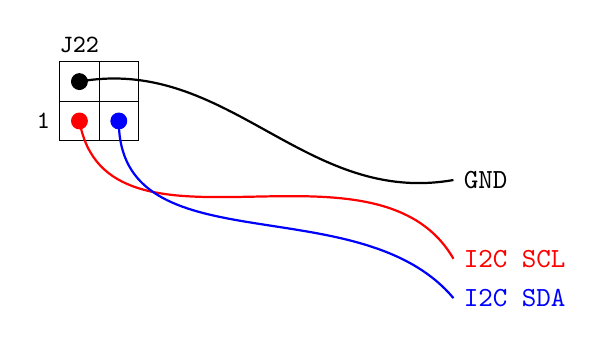
\begin{tikzpicture}
    % Pins
    \draw (0,0) rectangle (0.5,0.5);
    \draw (0.5,0) rectangle (1,0.5);
    \draw (0,-0.5) rectangle (0.5,0);
    \draw (0.5,-0.5) rectangle (1,0);

    % PCB labels
    \coordinate (A) at (0.25,0.5);
    \node at (A) [above] {\small\texttt{J22}};
    \coordinate (B) at (0,-0.25);
    \node at (B) [left] {\small\texttt{1}};

    % I2C GND
    \draw [black,fill] (0.25,0.25) circle [radius=0.1];
    \draw [thick] (0.25,0.25)
        to [out=10,in=190] (5,-1) node [right] {\texttt{GND}};

    % I2C SCL
    \draw [red,fill] (0.25,-0.25) circle [radius=0.1];
    \draw [red,thick] (0.25,-0.25) to [out=-80,in=120] (5,-2)
        node [right] {\texttt{I2C SCL}};

    % I2C SDA
    \draw [blue,fill] (0.75,-0.25) circle [radius=0.1];
    \draw [blue,thick] (0.75,-0.25) to [out=-90,in=130] (5,-2.5)
        node [right] {\texttt{I2C SDA}};
\end{tikzpicture}
\caption{Schematic for external \itwoc adapter setup.}
\label{fig:external_i2c}
\end{figure}

\subsubsection{Configure slave GBTx DB to use master SCA channel}
\label{sec:hardware-slave-sca}
This setup is required to program a slave via a master SCA channel.
In a typical scenario, the master is connected to a MiniDAQ so that programming
the slave using the MiniDAQ directly\footnote{
    MiniDAQ $\to$ master GBTx $\to$ slave GBTx.
}is possible.
Follow \autoref{fig:master-sca} to connect a slave GBTx to the SCA channel of a
master GBTx DB.

\begin{figure}[!ht]
\centering
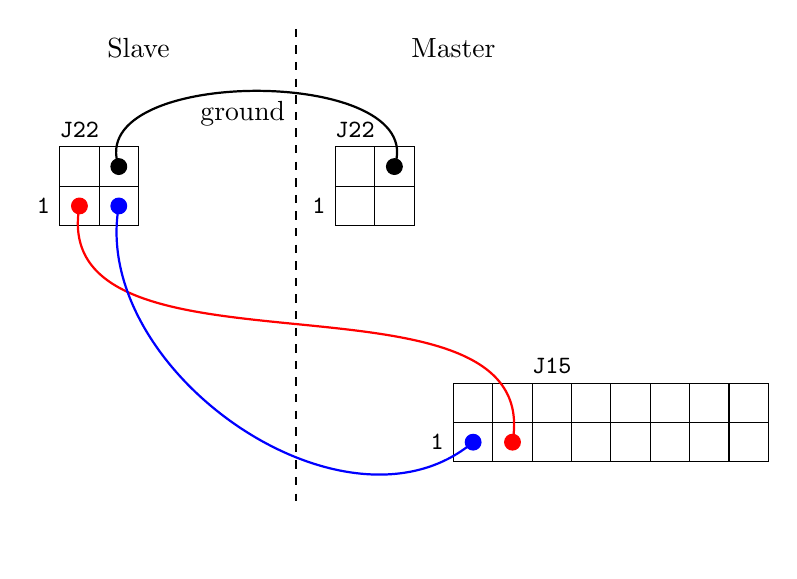
\begin{tikzpicture}
    % Separation
    \draw [thick,dashed] (0,3) to (0,-3);
    \coordinate (Slave) at (-2,3);
    \coordinate (Master) at (2,3);
    \node at (Slave) [below] {Slave};
    \node at (Master) [below] {Master};

    % Pins & labels on the slave
    \draw (-3,1) rectangle (-2.5,1.5);
    \draw (-2.5,1) rectangle (-2,1.5);
    \draw (-3,0.5) rectangle (-2.5,1);
    \draw (-2.5,0.5) rectangle (-2,1);
    \coordinate (A) at (-2.75,1.5);
    \node at (A) [above] {\small\texttt{J22}};
    \coordinate (B) at (-3,0.75);
    \node at (B) [left] {\small\texttt{1}};

    % Pins & labels on the master
    \draw (0.5,1) rectangle (1,1.5);
    \draw (1,1) rectangle (1.5,1.5);
    \draw (0.5,0.5) rectangle (1,1);
    \draw (1,0.5) rectangle (1.5,1);
    \coordinate (C) at (0.75,1.5);
    \node at (C) [above] {\small\texttt{J22}};
    \coordinate (D) at (0.5,0.75);
    \node at (D) [left] {\small\texttt{1}};
    % Another pin
    \draw (2,-1.5) rectangle (6,-2.5);
    \draw (2,-2) to (6,-2);
    \draw (2.5,-1.5) to (2.5,-2.5);
    \draw (3,-1.5) to (3,-2.5);
    \draw (3.5,-1.5) to (3.5,-2.5);
    \draw (4,-1.5) to (4,-2.5);
    \draw (4.5,-1.5) to (4.5,-2.5);
    \draw (5,-1.5) to (5,-2.5);
    \draw (5.5,-1.5) to (5.5,-2.5);
    \coordinate (E) at (3.25,-1.5);
    \node at (E) [above] {\small\texttt{J15}};
    \coordinate (F) at (2,-2.25);
    \node at (F) [left] {\small\texttt{1}};

    % Single grounding cable
    \draw [black,fill] (-2.25,1.25) circle [radius=0.1];
    \draw [black,fill] (1.25,1.25) circle [radius=0.1];
    \draw [thick,out=110,in=70] (-2.25,1.25)
    to node [below,xshift=-0.5em] {ground} (1.25,1.25);

    % 2x1 cross connector
    \draw [red,fill] (-2.75,0.75) circle [radius=0.1];
    \draw [red,fill] (2.75,-2.25) circle [radius=0.1];
    \draw [thick,red,out=-100,in=80] (-2.75,0.75) to (2.75,-2.25);
    \draw [blue,fill] (-2.25,0.75) circle [radius=0.1];
    \draw [blue,fill] (2.25,-2.25) circle [radius=0.1];
    \draw [thick,blue,out=-100,in=220] (-2.25,0.75) to (2.25,-2.25);
\end{tikzpicture}
\caption{Schematic for slave to master SCA setup.}
\label{fig:master-sca}
\end{figure}

\begin{leftbar}
    The black ground cable can be connected to any of the ground pin on the
    master GBTx DB.
\end{leftbar}

\subsubsection{Configure GBTx to use GBT-IC channel}
It might be useful to read/write \emph{individual} registers from/to a GBTx
board.
In this case, follow the \autoref{fig:gbt-ic} to flip the \texttt{configSelect}
switch.

\begin{leftbar}
    Normally this should be unjumped, because we use the SCA \itwoc channel from
    the master board to communicate with the slave.
\end{leftbar}

\begin{leftbar}
    Flip the \texttt{configSelect} switch will render the external \itwoc
    adapter ineffective.
    None of the GBTx register value is fused onto the board, so a GBTx board in
    our lab must always be programmed externally via \itwoc before flipping the
    switch.
\end{leftbar}

\begin{figure}[!ht]
\centering
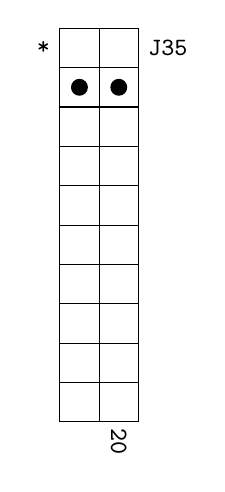
\begin{tikzpicture}
    % Pins
    \draw (0,0) rectangle (1,-5);
    \draw (0.5,0) to (0.5,-5);
    \draw (0,-0.5) to (1,-0.5);
    \draw (0,-1.5) to (1,-1.5);
    \draw (0,-2.5) to (1,-2.5);
    \draw (0,-3.5) to (1,-3.5);
    \draw (0,-4.5) to (1,-4.5);
    \draw (0,-1) to (1,-1);
    \draw (0,-2) to (1,-2);
    \draw (0,-3) to (1,-3);
    \draw (0,-4) to (1,-4);

    % PCB labels
    \coordinate (A) at (1,-0.25);
    \node at (A) [right] {\small\texttt{J35}};
    \coordinate (B) at (0,-0.25);
    \node at (B) [left] {\small\texttt{*}};
    \coordinate (C) at (0.75,-5.25);
    \node at (C) [rotate=-90] {\small\texttt{20}};

    % Pins that need to be connected
    \draw [black,fill] (0.25,-0.75) circle [radius=0.1];
    \draw [black,fill] (0.75,-0.75) circle [radius=0.1];
\end{tikzpicture}
\caption{
    Schematic for flipping the \texttt{configSelect} switch. A jumper should be
    used to connect the two pins marked above.
}
\label{fig:gbt-ic}
\end{figure}

\subsubsection{
    Configure GBTx DB in transmitter/transceiver and widebus/FEC mode
}
GBTx DBs can be configured to operate as a transmitter or a transceiver, with
a communication protocol of widebus or FEC, by hardware pins.
There are a total of 4 pins;
these related pins are shown in \autoref{fig:gbt-txrx}.

GBTx operations mode is completely determined by these 4 pins (corresponding to
4 bits). The 4-bit operation modes are listed in \nameref{appx:4bit}.

\begin{figure}[!ht]
\centering
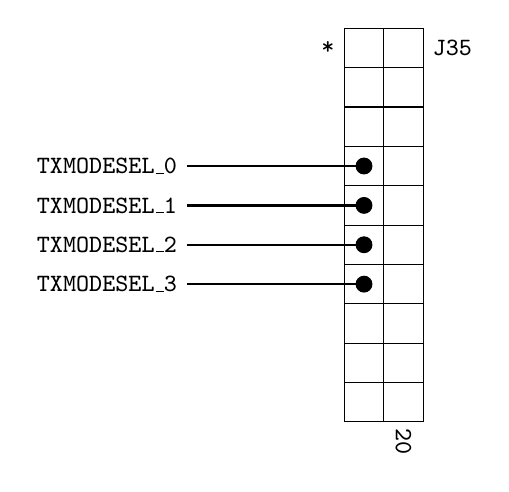
\begin{tikzpicture}
    % Pins
    \draw (0,0) rectangle (1,-5);
    \draw (0.5,0) to (0.5,-5);
    \draw (0,-0.5) to (1,-0.5);
    \draw (0,-1.5) to (1,-1.5);
    \draw (0,-2.5) to (1,-2.5);
    \draw (0,-3.5) to (1,-3.5);
    \draw (0,-4.5) to (1,-4.5);
    \draw (0,-1) to (1,-1);
    \draw (0,-2) to (1,-2);
    \draw (0,-3) to (1,-3);
    \draw (0,-4) to (1,-4);

    % PCB labels
    \coordinate (A) at (1,-0.25);
    \node at (A) [right] {\small\texttt{J35}};
    \coordinate (B) at (0,-0.25);
    \node at (B) [left] {\small\texttt{*}};
    \coordinate (C) at (0.75,-5.25);
    \node at (C) [rotate=-90] {\small\texttt{20}};

    % operation mode configuration pins
    \draw [black,fill] (0.25,-1.75) circle [radius=0.1];
    \draw [black,fill] (0.25,-2.25) circle [radius=0.1];
    \draw [black,fill] (0.25,-2.75) circle [radius=0.1];
    \draw [black,fill] (0.25,-3.25) circle [radius=0.1];

    \draw [thick] (-2,-1.75) to (0.25,-1.75);
    \node  at (-2,-1.75) [left] {\small\texttt{TXMODESEL\_0}};
    \draw [thick] (-2,-2.25) to (0.25,-2.25);
    \node  at (-2,-2.25) [left] {\small\texttt{TXMODESEL\_1}};
    \draw [thick] (-2,-2.75) to (0.25,-2.75);
    \node  at (-2,-2.75) [left] {\small\texttt{TXMODESEL\_2}};
    \draw [thick] (-2,-3.25) to (0.25,-3.25);
    \node  at (-2,-3.25) [left] {\small\texttt{TXMODESEL\_3}};
\end{tikzpicture}
\caption{
    Schematic showing all 4 related configuration pins.
    Note that the right column is a common ground.
    To switch a pin \emph{off}, connect it to a common ground pin.
}
\label{fig:gbt-txrx}
\end{figure}

\subsubsection{Reset GBTx ASIC}
Sometimes GBTx ASIC will not be properly reset by reprogramming, or it may have
erratic/unexpected behaviors.
In such case, a manual jumper reset can be performed on the GBTx DB to reset
GBTx ASIC.
Follow the \autoref{fig:gbtx-reset} to reset GBTx ASIC.

\begin{figure}[!ht]
\centering
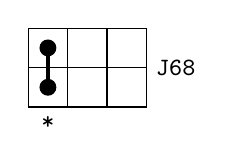
\begin{tikzpicture}
    % Pins
    \draw (0,0) rectangle (1.5,-1);
    \draw (0,-0.5) to (1.5,-0.5);
    \draw (0.5,0) to (0.5,-1);
    \draw (1,0) to (1,-1);

    % PCB labels
    \coordinate (A) at (1.5,-0.5);
    \node at (A) [right] {\small\texttt{J68}};
    \coordinate (B) at (0.25,-1);
    \node at (B) [below] {\small\texttt{*}};

    % Pins that need to be connected
    \draw [black,fill] (0.25,-0.75) circle [radius=0.1];
    \draw [black,fill] (0.25,-0.25) circle [radius=0.1];
    \draw [ultra thick] (0.25,-0.75) -- (0.25,-0.25);
\end{tikzpicture}
\caption{
    Schematic for resetting GBTx ASIC. A jumper should be used to connect the
    two pins marked above.
}
\label{fig:gbtx-reset}
\end{figure}


\subsection{DCB}
\subsubsection{Overview}
Our current setup consists of one master and one slave GBTx board.
When the slave is in widebus transceiver mode,
the master is connected to the MiniDAQ GBTx channel 3 (fiber 8),
and the slave can be connected to either GBT channel 0 (fiber 6) or channel 6
(fiber 11).
The master synchronizes its on-board clock to the signal from the MiniDAQ,
and propagates its clock signal to the slave.
The slave does not have an on-board clock,
and is configured to obtain clock signal externally.

When the slave is in widebus transmitter mode,
again the master is connected to channel 3,
and the slave can be connected to any of the MiniDAQ channel 6-11
(physical fiber 11, 9, \ldots, 1).
We will use these channels to connect to upcoming DCB boards.

The master \itwoc port is connected to an external USB device.
The slave \itwoc port is connected to the master.
Both are set to be programmed by the \itwoc channel,
rather than GBT-IC channel.

The current setup is capable of:
\begin{enumerate}
    \item Program the slave GBTx board with MiniDAQ directly.
    \item Read/Write the register value of the master GBTx board with GBT-IC
        specification on the MiniDAQ.
    \item Do PRBS tests from MiniDAQ to the slave, with slave configured in
        either transceiver or transmitter mode, then back to the MiniDAQ.
        The master is also required\footnote{
            The master GBTx is also connected to the MiniDAQ with a different
        channel, to provide reference clock to the slave.}
        as the slave can only obtain its reference clock from the master.
\end{enumerate}


\section{Software setup}
\subsection{Program master GBTx with external \itwoc adapter}
Before proceed, follow the instruction on \autoref{sec:hardware-ext-i2c} to
configure the hardware first.
As said in the previous section, the master GBTx board must be programmed via an
external \itwoc adapter first.
A Windows 7 computer on the rack is used. The \textbf{GBTX programmer} is
located at:

\begin{lstlisting}
DT_Rack\GBTx_programmer\GBTxProgrammer.jar
\end{lstlisting}

\begin{figure}[ht]
    \centering
    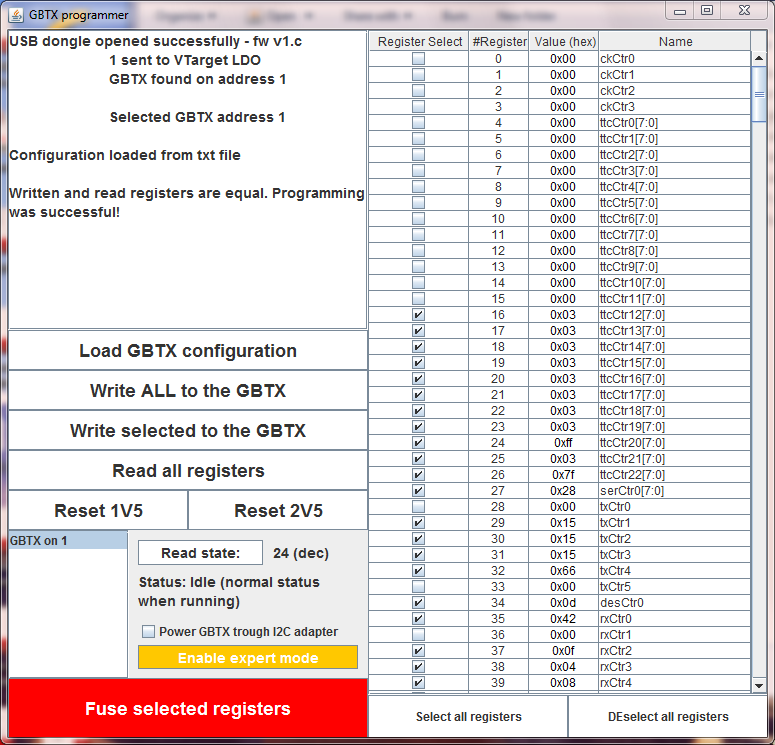
\includegraphics[width=0.9\textwidth]{res/gbtx_programmer_v1_ui.png}
    \caption{A typical UI for GBTX programmer.}
    \label{fig:gbtx-programmer-ui}
\end{figure}

Launch the programmer, a typical UI is shown in
\autoref{fig:gbtx-programmer-ui},
Click \textbf{Load GBTX configuration} and load a configuration file, which is
located at:

\begin{lstlisting}
Documents\master.txt
\end{lstlisting}

Then click \textbf{Write ALL to the GBTX}. Check the returned message to make
sure everything works (supposedly).
Now click \textbf{Read state}.
If the master GBTx is configured correctly and is connected to a working
MiniDAQ, the return value should be:

\begin{lstlisting}
24 (dec): Idle (normal status when running)
\end{lstlisting}

\subsection{Check communication between master GBTx and MiniDAQ}
After programming the master GBTx board and verifying the return value, we can check
the communication between the GBTx and the MiniDAQ with \textbf{GBT Client}.

\begin{figure}[ht]
    \centering
    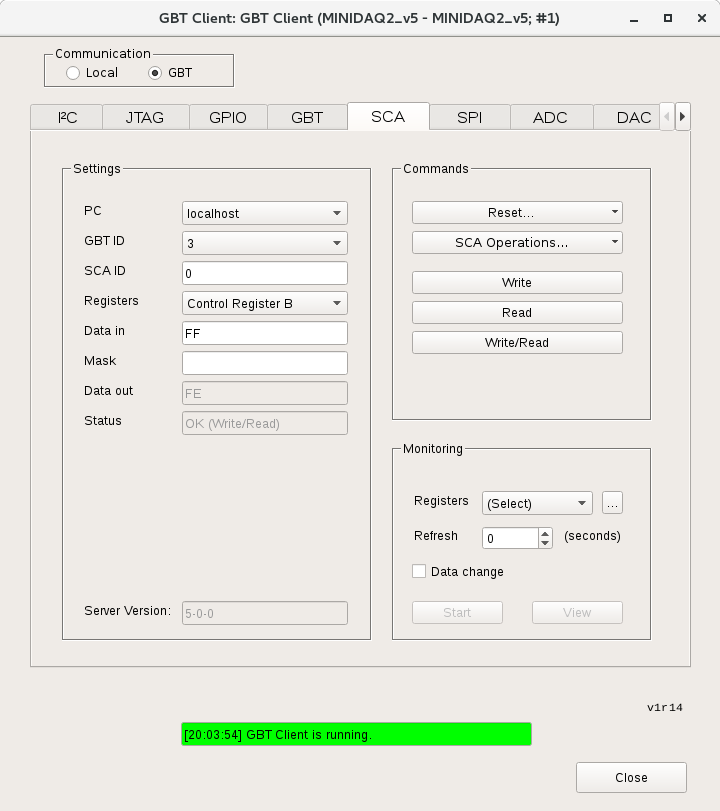
\includegraphics[width=0.9\textwidth]{res/gbt_client_master_gbt_sca_test.png}
    \caption{A typical UI for GBT Client, SCA tab.}
    \label{fig:sca-ui}
\end{figure}

Here we need to use the Linux server on the rack.
To launch that program, locate the \textbf{gedi} panel. Under
\textbf{LHCB framework},
click the \textbf{GBT Client}.
Choose \textbf{GBT} option under the \textbf{Communication} tab.
Navigate to \textbf{SCA} tab.

To check whether the link between GBTx and MiniDAQ is successfully established,
configure the parameters as shown in \autoref{fig:sca-ui},
changing \textbf{GBT ID} according to one's setup.

Now click \textbf{Write/Read}.
The \textbf{Data out} field should have a value of ``\texttt{FE}'', and the
\textbf{Status} should be ``OK (Write/Read)''.

\begin{leftbar}
    \textbf{GBT ID} corresponds to the physical optical link that is connected
    to the master GBTx board.
    Recall that in our setup, the master is connected to optical fiber 8, which
    is mapped to GBT channel 3.
\end{leftbar}

\begin{leftbar}
    There are only 4 \textbf{Registers}.
    All 4 registers work, the ``Control Register B'' is chosen for no apparent
    reason.
    What matters is the return value should be consistent with our expectation.
\end{leftbar}

\subsection{Program individual registers of slave GBTx}
\label{sec:software-slave-individual}
Before proceed, follow \autoref{sec:hardware-slave-sca} to set up hardware.
Again we use \textbf{GBT Client} to program individual registers of the slave
GBTx.
Configure the parameter as shown in \autoref{fig:gbt-i2c}.

\begin{figure}[ht]
    \centering
    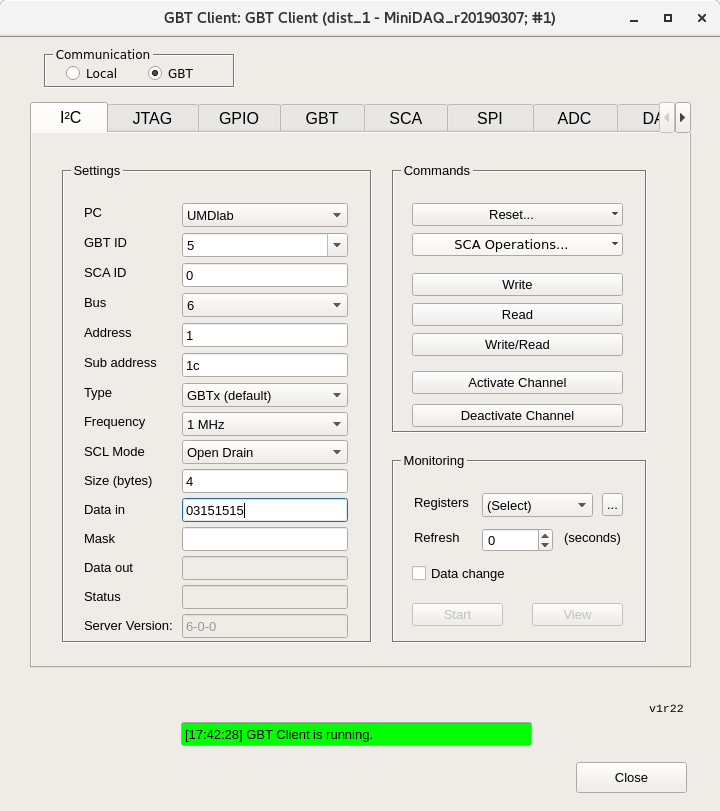
\includegraphics[width=0.9\textwidth]{res/gbt_client_slave_gbt_i2c_test.png}
    \caption{Correct parameters to configure GBT \itwoc tab.}
    \label{fig:gbt-i2c}
\end{figure}

\begin{leftbar}
    If the \textbf{Write} command failed, try \textbf{Activate Channel} first.
\end{leftbar}

\begin{leftbar}
    \textbf{Address} corresponds to GBTx index, which is configured via an
    onboard DIP switch. Default to 1.
\end{leftbar}

\begin{leftbar}
    Recall that 1 \emph{Byte} is 8 \emph{bits}, and 1 Byte corresponds to a
    2-digit hex number.
\end{leftbar}

\begin{leftbar}
    Notice in the \textbf{Data out} field, the last 3 numbers are the same.
    This is a requirement in the GBT specification that the configuration
    registers must be triplicated to minimize error.
\end{leftbar}

\subsection{Program slave GBTx with configuration files}
Configure the parameter as shown in \autoref{fig:gbt-file}.

\begin{figure}[ht]
	\centering
    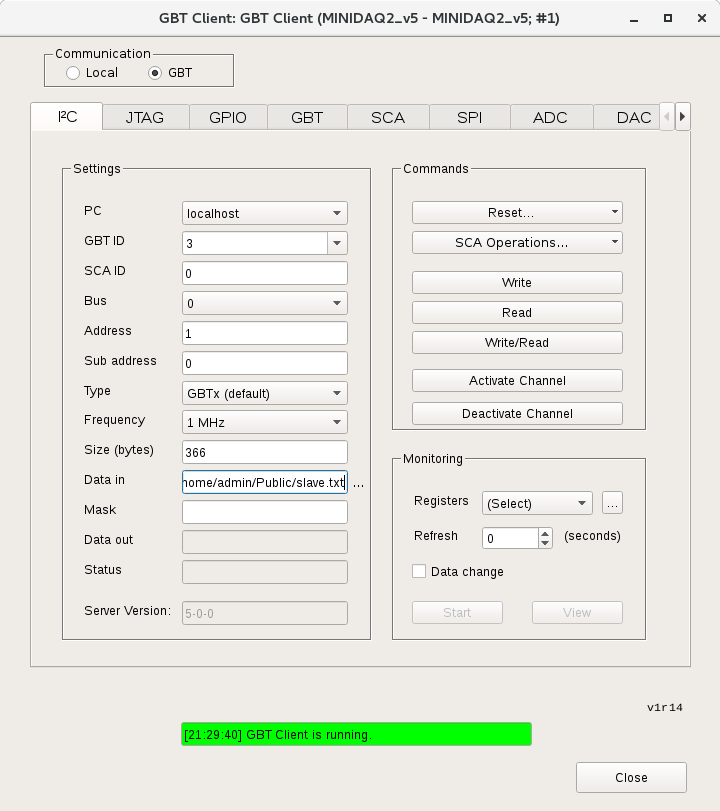
\includegraphics[width=0.9\textwidth]{res/gbt_client_slave_program_via_config_file.png}
	\caption{Parameters to program slave GBTx with a configuration file.}
	\label{fig:gbt-file}
\end{figure}

The configuration file should be supplied to the \textbf{Data in} field with the
following syntax:
\begin{minted}[frame=single]{powershell}
file:<path_to_configuration_file>
\end{minted}

The actual configuration file is located at:
\begin{minted}[frame=single]{powershell}
/home/admin/Public/slave.txt
\end{minted}

\begin{leftbar}
    This is equivalent to program the slave with an external \itwoc adapter.
    The advantage of doing this way is we don't need to remove the \itwoc
    adapter from the master.
    In other words, once the hardware setup is done, we don't have to touch them
    anymore; whereas if we program both master and slave with an \itwoc adapter,
    it must be moved around between the master and the slave.
\end{leftbar}


\newpage \appendix
\section*{Appendices}
\addcontentsline{toc}{section}{Appendices}
\renewcommand{\thesubsection}{\Alph{subsection}}
\subsection{Fix ``Waiting for a GBT server to run''}
Sometimes when we launch the \textbf{GBT Client}, it would claim that it is
``Waiting for a GBT server to run''.
Take this warning literally: It means that currently there is no GBT server that
is alive.
The fix is easy: fire up a terminal, and type in ``\texttt{GbtServ}''.

\subsection{Bypass components in GBT data path}
As shown in \autoref{fig:gbt-data-path}, we can bypass components in GBT
input/output path.

\begin{figure}[ht]
    \centering
    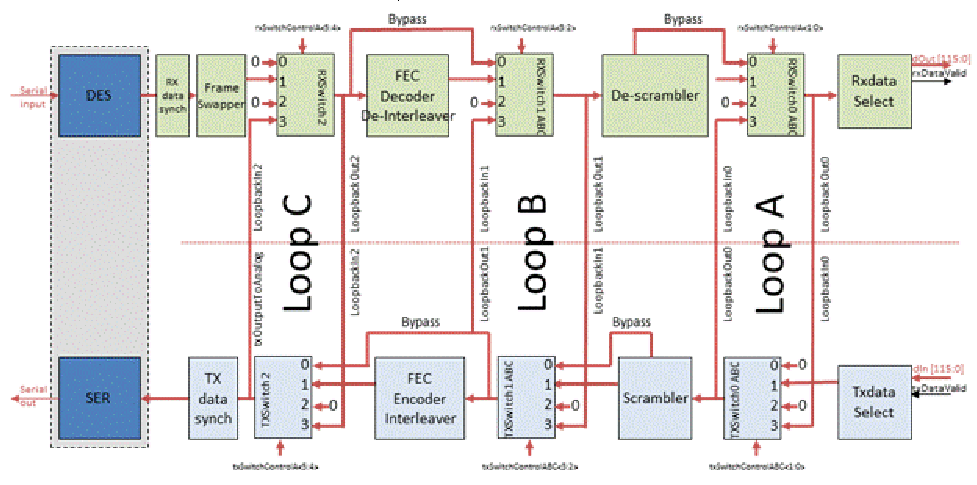
\includegraphics[width=\textwidth]{res/gbtx_data_path_block_diagram.pdf}
    \caption{GBT data path. Stolen from LHCb \emph{GBTX manual}.}
    \label{fig:gbt-data-path}
\end{figure}

The register \texttt{0x1c} and 3 subsequent registers control the output path;
\texttt{0x2d} controls the input path.
Each of the paths have 3 configurable selectors, each has 4 operations modes
($0_{10} - 3_{10}$, which translate to $0_2 - 11_2$)\footnote{
    The subscript indicates the base.
}.
According to \autoref{fig:gbt-data-path}, the control sequence should be given
in:

\begin{lstlisting}
TXSwitch2 -> TXSwitch1 -> TXSwitch0
\end{lstlisting}

Here is an example.
Let us consider the Tx normal operating case (i.e.\ all 3 switches are
configured to 1). We have:
\begin{align*}
    \underbrace{1_{10}}_{\text{\tiny ~TXSwitch2~}}
    &\underbrace{1_{10}}_{\text{\tiny ~TXSwitch1~}}
    \underbrace{1_{10}}_{\text{\tiny ~TXSwitch0~}} \\
    &\symbolwithin{\Downarrow}{\text{\tiny ~TXSwitch0~}} \\
    \underbrace{01_{2}}_{\text{\tiny ~TXSwitch2~}}
    &\underbrace{01_{2}}_{\text{\tiny ~TXSwitch1~}}
    \underbrace{01_{2}}_{\text{\tiny ~TXSwitch0~}} \\
\end{align*}

To convert binary $010101_2$ to hexadecimal, we left pad the result with 2
additional 0's: $0001,0101_2$. The end result is $15_{16}$.

\begin{leftbar}
    $15_{16}$ is exactly the last 3 bytes in \textbf{Data out} field in
    \autoref{fig:gbt-i2c}.
    This is not a coincidence.
\end{leftbar}

\begin{leftbar}
    Recall that each 4 digits in binary exactly correspond to 1 digit in
    hexadecimal.
\end{leftbar}

\subsection{PRBS tests}
``PRBS'' stands for pseudo-random-bit-sequence.

\paragraph{Test 1.}
This test instructs slave GBTx to transmit self-generated PRBS data, instead of
elink data.
Follow the following steps:
\begin{enumerate}
    \item Configure the GBTx slave to send PRBS data. Write ``03151515'' to
        slave register \texttt{0x1c}, setting size to 4.
    \item Go to the top MiniDAQ hardware panel, click on \textbf{PRBS}.
    \item In the \textbf{PRBS} panel, click in sequence:
        \textbf{Stop All Generators} $\to$ \textbf{Stop All Checkers} $\to$ 
        \textbf{Reset All Counters} $\to$
        \textbf{Start All Generators} $\to$ \textbf{Start All Checkers} $\to$
        \textbf{Start All Counters}.
\end{enumerate}

The result should be the same as shown in \autoref{fig:prbs-test1}.

\begin{figure}[ht]
    \centering
    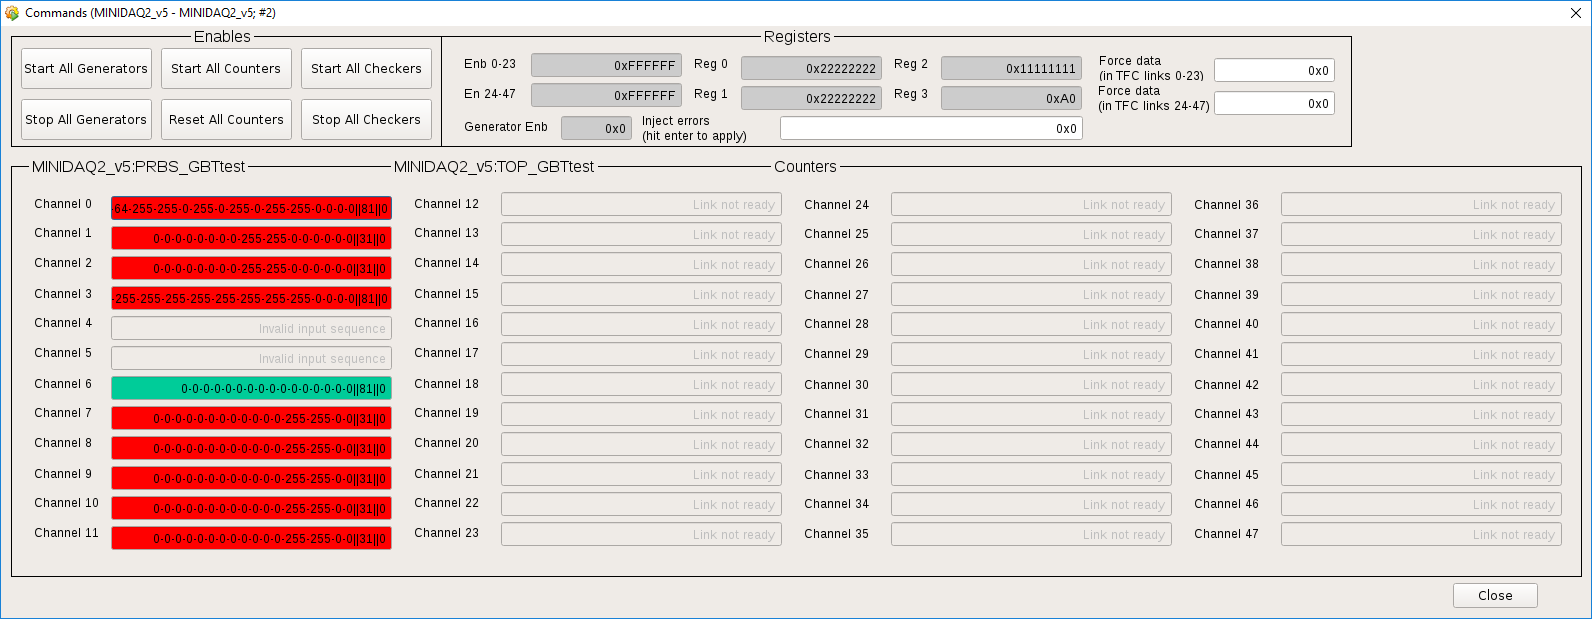
\includegraphics[width=\textwidth]{res/prbs_test1.png}
    \caption{Expected result for PRBS test 1.}
    \label{fig:prbs-test1}
\end{figure}

\begin{leftbar}
    Channel 6 (optical fiber 11, which is connected to slave GBTx) should go
    green and show a bunch of 0s.
    These 0s are the PRBS nibbles (7 bits) each from the GBT.
\end{leftbar}

\begin{leftbar}
    Channel 7 or any other channels should go red and show a lot of errors,
    because these are receiving the FE data in loopback and not the ``correct''
    random data that the checkers are expecting.
\end{leftbar}

After replacing the loaned MiniDAQ board with our original board, we no longer
can reproduce the exact behavior:
All loopback channels go green, instead of error out.
We deem it acceptable, at least for the time being.

\paragraph{Test 2.}
This is a loopback test, bypassing GBTx ASIC.
Follow the following steps:
\begin{enumerate}
    \item Configure the GBTx slave to send PRBS data. Write ``00171717'' to
        slave register \texttt{0x1c}, setting size to 4.
    \item Go to the top MiniDAQ hardware panel, click on \textbf{PRBS}.
    \item In the \textbf{PRBS} panel, click in sequence:
        \textbf{Stop All Generators} $\to$ \textbf{Stop All Checkers} $\to$
        \textbf{Reset All Counters} $\to$
        \textbf{Start All Generators} $\to$ \textbf{Start All Checkers} $\to$
        \textbf{Start All Counters}. (same as in test 1).
\end{enumerate}

The result should be the same as shown in \autoref{fig:prbs-test2}.

\begin{figure}[ht]
    \centering
    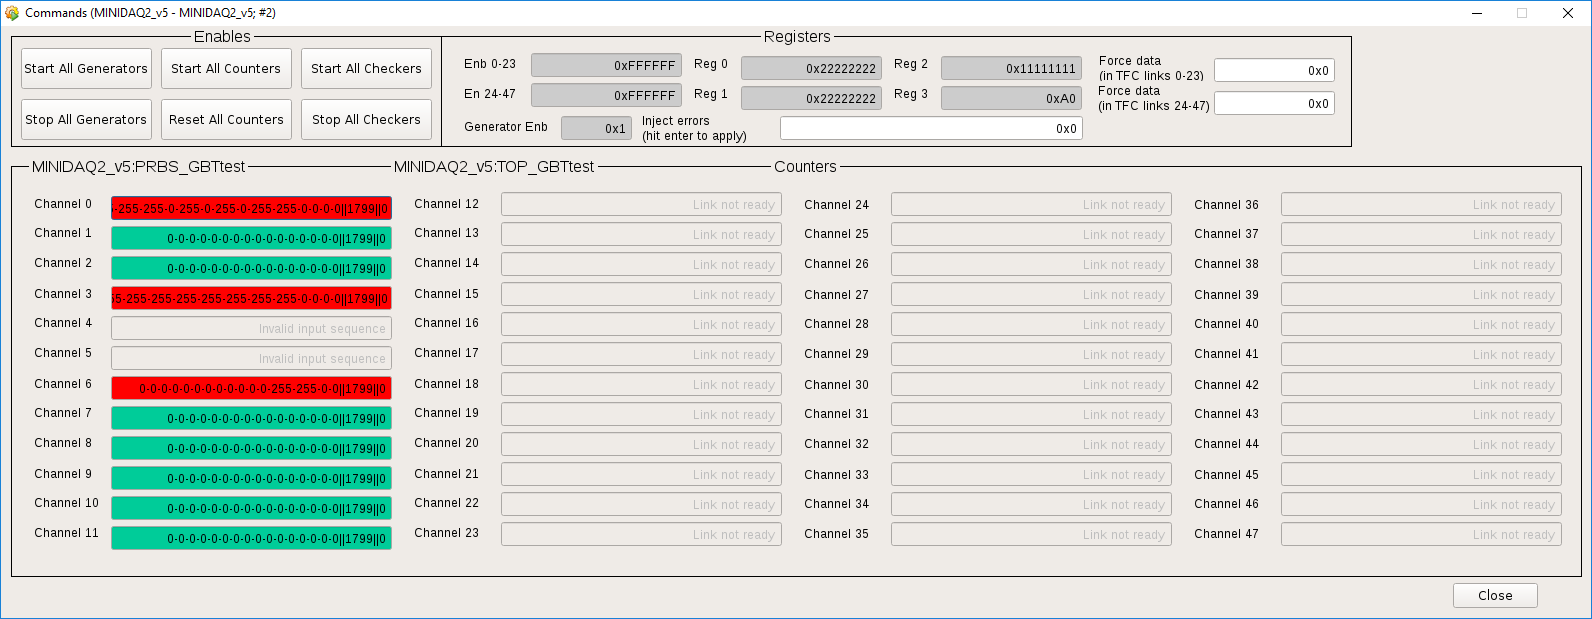
\includegraphics[width=\textwidth]{res/prbs_test2.png}
    \caption{Expected result for PRBS test 2.}
    \label{fig:prbs-test2}
\end{figure}

\begin{leftbar}
    All channels that are in loopback should go green: Now the PRBS data is
    generated inside FPGA, it overwrites the FE data and goes back in loopback
    to the checkers.
\end{leftbar}

\begin{leftbar}
    Channel 6  shows counting errors on two nibbles.
    The reason, according to expert Federico Alessio, is the clock-crossing
    domain inside the GBTx chip that generates errors in the loopback path,
    which is a feature of the GBT.
\end{leftbar}

\begin{leftbar}
    The increasing counter to the right of each line in the PRBS block is the
    number of seconds since we started the counters.
\end{leftbar}

\begin{leftbar}
    To have again FE data we need to disable the generators:
    \textbf{Stop All Generators} in the \textbf{PRBS} panel.
\end{leftbar}

\begin{leftbar}
    When the PRBS panel shows ``Input data not valid'', it means that the
    system is generating all 0s.
\end{leftbar}

\subsection{GBTx operation modes} \label{appx:4bit}
\begin{center}
    \begin{tabular}{ccc}
        \toprule
        Enconding/Bus mode & Transceiver mode & MODE [3:0] \\
        \midrule
        FEC & Simplex TX  & 0000 \\
        FEC & Simplex RX  & 0001 \\
        FEC & Transceiver & 0010 \\
        FEC & Test        & 0100 \\
        WideBus & Simplex TX  & 0100 \\
        WideBus & Simplex RX  & 0101 \\
        WideBus & Transceiver & 0110 \\
        WideBus & Test        & 0111 \\
        \bottomrule
    \end{tabular}
    \captionof{table}{
        GBTx operation modes (dubbed as ``Transceiver modes'').
        Stolen from LHCb \emph{GBTX manual}.
    }
    \label{tab:gbtx-modes}
\end{center}


\end{document}
